\documentclass[dvipdfmx, a4paper, 14Q, fleqn]{jreport}
\usepackage{../preamble/preamble_TeXManual}
\begin{document}
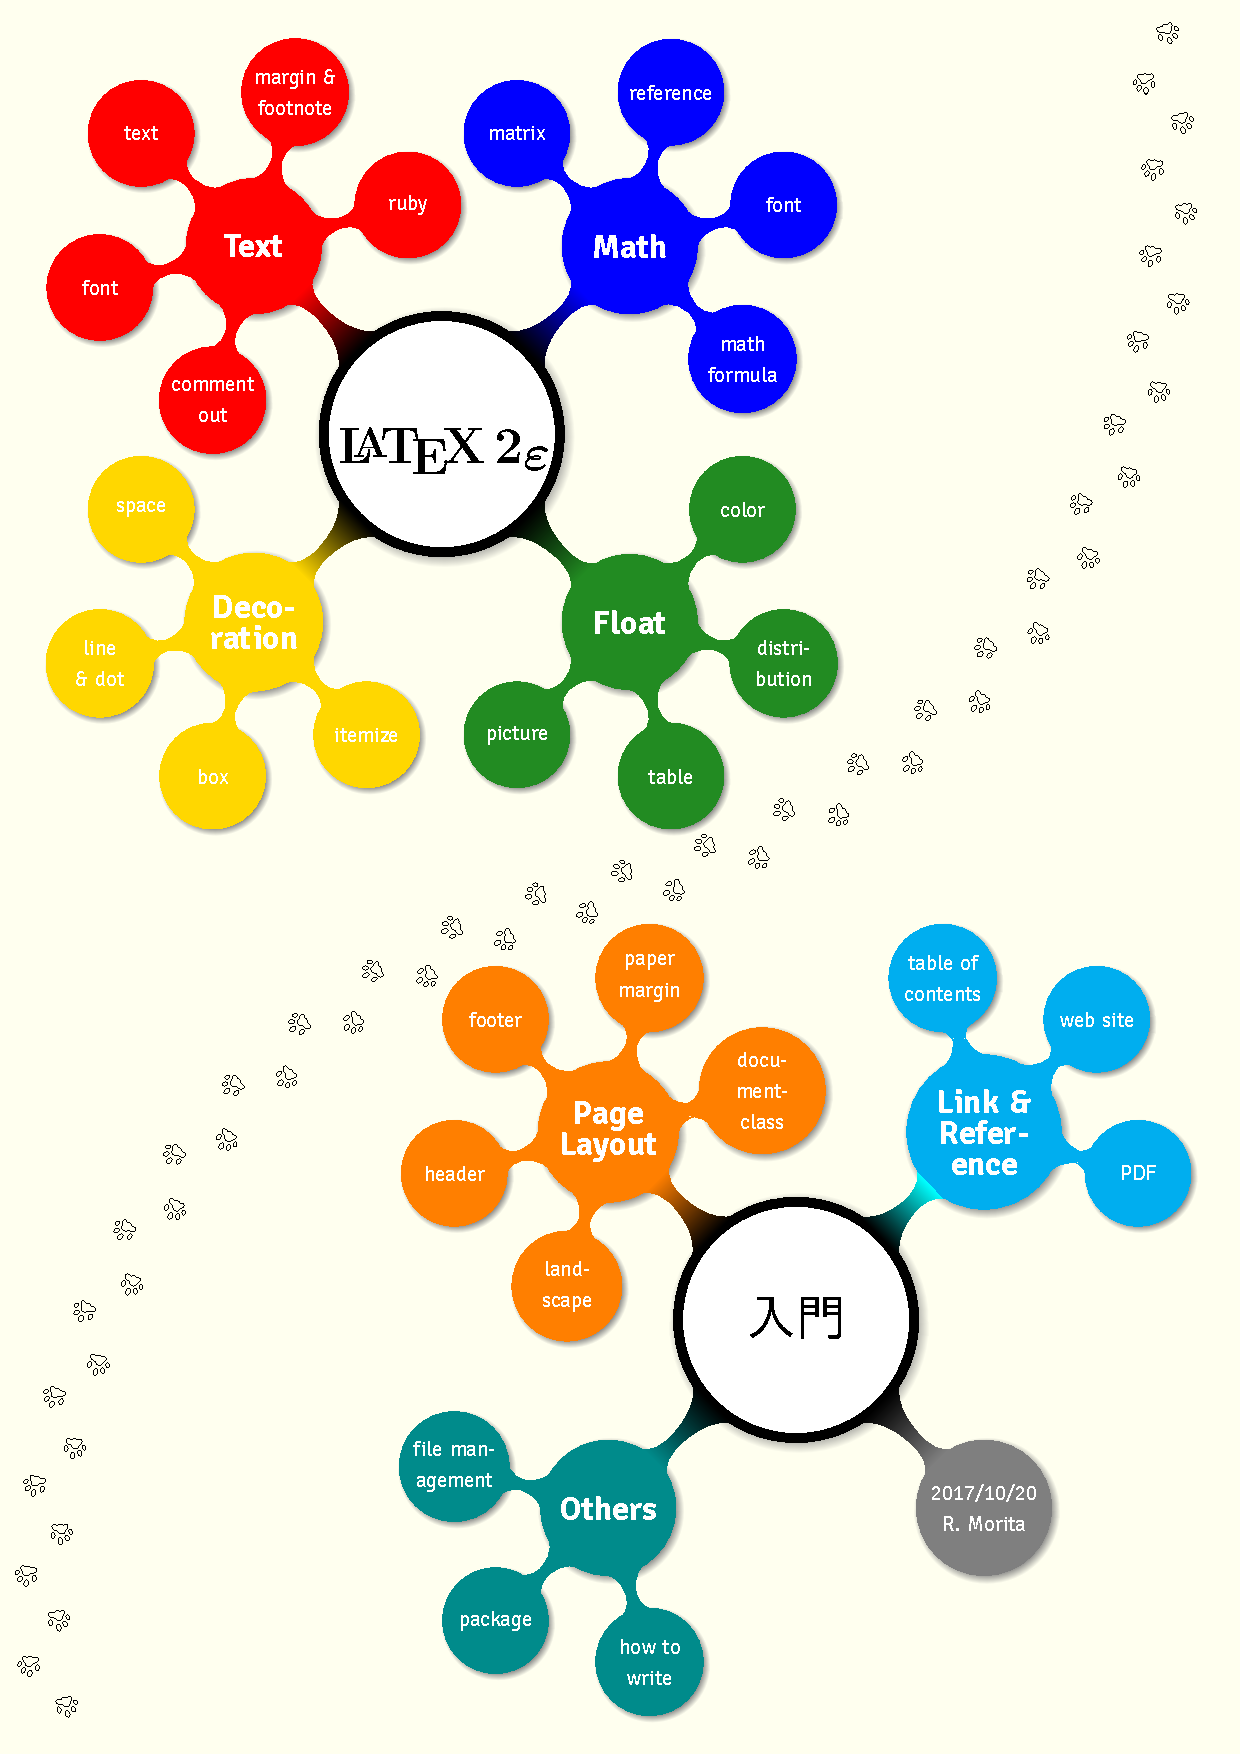
\includepdf[offset = 0mm -14mm]{../titlepage/titlepage_mindmap.pdf}
\subimport{../chapters/chapter0_introduction/}{introduction}
\tableofcontents
\subimport{../chapters/chapter1_preparation/}{before_making_document}
\subimport{../chapters/chapter2_plane_text/}{how_to_write_plane_text}
\subimport{../chapters/chapter3_environment/}{about_environment}
\subimport{../chapters/chapter4_math/}{math_formula}
\subimport{../chapters/chapter5_pictures/}{about_pictures}
\subimport{../chapters/chapter6_tables/}{about_tables}
%\subimport{../chapters/chapterx7_macros/}{how_to_make_macros}			%未実装
\subimport{../chapters/chapter8_references_contents_links/}{references_contents_links}		%索引追加
\subimport{../chapters/chapterx_pagelayout/}{pagelayout}			%titlesec追加
\subimport{../chapters/chapterx_fonts/}{about_europian_fonts}	%書き足し予定(未定)
\subimport{../chapters/chapterx_fonts/}{about_japanese_fonts}	%書き足し予定(未定)
%\subimport{../chapters/chapterx_about_bibliography/}{how_to_write_bibliography} 	%未実装
\subimport{../chapters/chapterx_file_management/}{file_management}
\subimport{../chapters/chapterx_right_words/}{how_to_write_right_words}		%随時更新
\subimport{../chapters/chapterx_useful_packages/}{useful_packages} 			%随時更新
\subimport{../chapters/chapterx_others/}{other_topics}
\subimport{../bibliography/}{bibliography}
\end{document}

%physics・タイトルのデザインは書きたい

%以下実装未定
%mathabx, bbm, listing, 縦書き
%\subimport{../chapters/chapter_/}{TikZ}
%\subimport{../chapters/chapter_/}{tcolorbox}
%\subimport{../chapters/chapter_/}{スタイルファイルの作り方}
%\subimport{../chapters/chapter_/}{オンラインでTeXをする}
%\subimport{../chapters/chapter_/}{PythonTeX}